\documentclass[12pt]{article}

%Allgemeine Einstellungen

%Abstände
\usepackage[a4paper,left=3cm,right=3cm,top=3cm,bottom=3.5cm,headsep=12pt]{geometry}%Bottom extra 0.5cm für Footer

%Deutsches Sprachpacket
\usepackage[german,ngerman]{babel}

%Times New Roman
\usepackage{mathptmx}

%Titelseite einbinden
\usepackage{pdfpages}

%1.5-Zeilenabstand
\usepackage[onehalfspacing]{setspace}

%Stil der Überschriften, siehe ueberschriften.sty
\usepackage[numeric]{ueberschriften}

%Stil des Inhaltsverzeichnisses, siehe inhaltsverzeichnis.sty
\usepackage[numeric]{inhaltsverzeichnis}

%Abkürzungsverzeichnis, siehe abk_verzeichnis.sty
\usepackage{abk_verzeichnis}

%Stil der Fußzeilen, siehe fusszeilen.sty
\usepackage{fusszeilen}

%Literaturverzeichnis und Zitate, siehe literatur.sty
\usepackage{literatur}

%Stil für Header und Footer, siehe header_footer.sty
%Wenn nicht erwünscht, müssen auch die Befehle \frontmatter, \mainmatter auskommentiert werden
\usepackage{header_footer}

%Stile für Code-Ausschnitte, siehe codes.sty
\usepackage{codes}

%Stile für Anhänge, Bilder, ...
\usepackage{anhang}

%Silbentrennung (manche Worte werden am Zeilenende nicht getrennt, diese müssen dann nachgetragen werden)
\usepackage[T1]{fontenc}
\hyphenation{öf-fent-lich-en}

%DEBUGGING (Zeigt Boxen an)
%\usepackage{showframe}

\begin{document}

\renewcommand{\mytitle}{Governanceethik und\\moralische Anreize}%Titel für oben links
\renewcommand{\myauthor}{Lennart Schulte-Kellinghaus,\\Timo Stovermann}%Name für unten links
\renewcommand{\headheight}{27pt}%Bei Mehrzeiligem Titel muss Headerhöhe angepasst werden


\includepdf[pages={1-}]{titelseite.pdf}

\frontmatter%Stil des Headers/Footers ändern

\pagenumbering{Roman}

\addcontentsline{toc}{part}{Abkürzungsverzeichnis}%Abk-Verz. ins Inhaltsverzeichnis
\printabbreviations%abk_verzeichnis.sty
\clearpage

\renewcommand{\plaintitle}{Inhaltsverzeichnis}%Titel für oben Rechts
%Defbox, damit gepunktete Linie bis zur Zahl geht
{\def\makebox[#1][#2]#3{#3}%
	\tableofcontents
}

\addtocontents{toc}{\vspace{24pt}}%Freiraum im ToC

\clearpage
\mainmatter%Stil des Headers/Footers ändern
\pagenumbering{arabic}

\part{Einleitung und begriffliche Grundlagen}
Ethik spielt in Unternehmen eine immer größer werdende Rolle. Im Kontrast zum 20. Jahrhundert, als beispielsweise hohe Emissionswerte eines Unternehmens kaum Beachtung gefunden haben, legen Unternehmen heute mehr Wert auf klimaneutrales Arbeiten. Genauso hat sich die Lohnzahlung in den letzten Jahren verändert. Ein gleicher Lohn für Männer wie Frauen war lange Zeit keine Selbstverständlichkeit. Diese beiden Veränderungen sind neben vielen anderen maßgeblich durch Ethik bestimmt. In wie fern die Ethik und gesellschaftliche wie moralische Aspekte die Governance eines Unternehmens beeinflussen, soll hier kurz erörtert werden.

\section{Governance Begriff}
Unter Governance versteht man das steuern bzw. leiten und es wird mit dem Begriff versucht neue, nicht hierarchischen Formen der Steuerung und des Regierens in Netzwerken zu beschreiben.\citebibshort{governanceDef}{}{Vgl. } Im unternehmerischen Umfeld spricht man von Corporate Governance, und beschreibt in einem Unternehmen den rechtlichen und faktischen Ordnungsrahmen für die Leitung und Überwachung.\citebibshort{defCO}{}{Vgl. } Durch Corporate Governance soll versucht werden, Spielräume und Motivationen für die Akteure in einem Unternehmen rechtlich und faktisch zu arrangieren, damit die Akteure sich wohl fühlen und opportunistisches Verhalten eingeschränkt wird.\footnote{Vgl. ebd}

\section{Ethik und Moral im Kontext der Governance}
Die Ethik bildet die philosophische Grundlage für moralische Vorstellungen und ist praxisorientiert, das heißt ihr Ziel ist es, Aktuere moralisch Handeln zu lassen.\citebibshort{ethikDef}{S.11}{Vgl. } Sie bildet sich aus der Kombination von normativen Vorschriften, rechtlichen Rahmenbedingungen und den persönlichen Ansichten eines Individuums.\footnote{Vgl. ebd.} Daraus folgt, dass Ethik im Sinne des Eigeninteresses nicht mit Ethik im Sinne des Gemeinwohles gleichzusetzen ist. Das Eigeninteresse kann sich dabei sowohl auf natürliche als auch auf juristische PErsonen beziehen. Im Prozess der Governance spielen ethische Fragestellungen eine bedeutende Rolle, um die Ziele der o.g. Corporate Governance zu erreichen.

\section{Funktionssysteme und Organisationssysteme}
Wenn wir eine beliebige wirtschaftliche Transaktion betrachten, so hat diese verschiedene Dimensionen. Eine Bestellung von Waren bei einem langjährigen Lieferpartner hat Hintergründe aus ökonomischen, rechtlichen und moralischen Überlegungen. Der Grund dafür liegt in der funktionalen Differenzierung der Gesellschaft. Unsere Gesellschaft besteht aus vielen einzelnen Funktionssystemen, die jeweils eine bestimmte Funktion für die Gesellschaft übernehmen.\citebibshort{funksysDef}{S.49}{Vgl. }\\
Doch wie können verschiedenartige Systeme in einem Unternehmen zusammenwirken, wenn sie doch alle nur ihre eigene Sichtweise verstehen? Dazu definiert Wieland das Konstrukt Unternehmen selbst als Organisationssystem, welches durch die Governancestrukturen \glqq polylinguale Diskurse\grqq\citebibshort{wieland1}{S.8}{} ermöglicht.

\part{Die Treiber moralischen Handelns}
Nun bleibt aber die Frage, wodurch moralisches Verhalten in Governancestrukturen getrieben wird. Dazu gibt es verschiedene Ansätze, die sich entweder in die Kategorie der monistischen Ansätze, bei denen Ethik und Ökonomik letztendlich die gleiche Problemstellungen behandeln, oder in die KAtegorie der dualistischen Ansätze, bei denen Ethik und Moral eigenständige Dimensionen des menschlichen Verhaltens darstellen, einordnen.\citebibshort{homann}{S.3}{Vgl. }

\section{Monistische Sichtweise}z
Nach der monistischen Ansicht sind die Problemstellungen von Ethik und Ökonomik deckungsgleich. Die hauptsächliche Kritik an der dualistischen Theorie liege dabei in der grundsätzlichen Verschiedenheit der Moral und der Ethik, da durch diese eine Zusammenführung der beiden Pole nur unter massiven Abstrichen für mindesten einen der beiden möglich werde.\footnote{Vgl. ebd.}\setlength{\footnotemargin}{5mm} Zudem seien keine Regeln für das Zusammenspiel von Ethik und Ökonomik definiert, wodurch sich diesbezügliche Entscheidungen oft spontan aus der Situation ergäben.\footnote{Vgl. ebd.}
\\
Neben diesen Kritikpunkten an der dualistischen Ansätzen argumentiert der Soziologe Amitati Etzioni, dass moralisches Verhalten nicht auf ein Anreizsystem zurückführbar sei.\citebibshort{etzioni}{S.135. ff.}{Vgl. } Vielmehr vertritt er den Standpunkt, dass ethikkonformes Verhalten immer durch moralische und vor allem ökonomische Erwartungen bestimmt sei, wobei die Anreize sogar nur ökonomischer Natur seien.\citebibshort{wieland1}{S.5}{Vgl. } Daraus lässt sich schließen, dass für Etzioni sämtliche moralischen Handlungen von Unternehmen wie Privatpersonen in letzter Instanz auf materiellen Motivationen beruhen. Dies könnte zum Beispiel ein \textit{grünes Markenimage} oder eine Konformität mit aktuellen sozio-politischen Entwicklungen sein, wie die Einführung einer Frauenquote.
\\
Der Ökonom Karl Homann verteidigt den noch radikaleren monistischen Standpunkt, dass Ökonomisches Handeln in sich schon ethisch bzw. moralisch richtig sei.\citebibshort{homann}{S.5}{Vgl. } Die Begründung dafür sieht er in der Unvermischbarkeit verschiedener Einzelwissenschaften beim Lösen ökonomischer Fragen. Seine Methapher des Eisbergs, bei dem 1/7 glänzende Moral und 6/7 die versteckten ökonomischen Anreize sind, erschien uns sehr vielsagend. In ökonomischen Entscheidungsprozessen manifestieren sich ethische Überlegungen und Handlungsempfehlungen.\footnote{Vgl. ebd} Um diese Theorie umzusetzen, wird der Begriff der ökonomischen Vorteile um ethische Aspekte wie gutes Leben und Selbstverwirklichung ergänzt, langfristiger angesetzt und stärker auf die Interaktion von Märkten und Akteuren fokussiert.\footnote{Vgl. ebd. S.6} Eine Konsequenz daraus ist, dass die Handlungsregeln nicht etwa durch gesellschaftliche Moralvorstellungen vorgegeben werden, sondern sich aus dem ökonomischen Problem selbst hervorgehen.\footnote{Vgl. ebd.} Damit wird direkt dem Problem von ökonomisch unmöglichen moralischen Anforderungen ausgewichen, da solche Anforderungen letztendlich nur “Moralisieren, Appelieren und [...] Schlundzuweisungen”\citebibshort{homann}{S.4}{} oder anders ausgedrückt “Rauschen in der Wirtschaft”\citebibshort{wieland1}{S.12}{} erzeugen.
\\
Ein aus unserer Sicht sehr fragwürdiges Beispiel dafür, dass die “Ökonomik [...] Empfehlungen zur Lösung ethischer Probleme [gebe]\citebibshort{homann}{S.7}{}, wird von Karl Homann angeführt. Er behauptet, dass die angebliche Ausbeutung der Entwicklungsländer durch die Industriestaaten primär gar nicht auf eine Ausbeutung zugunsten letzterer abziele, sondern auf auf einer positiven Entwicklung aller Beteildigten, da Besserungen in armeren PArtner-Ländern den Industriestaaten letztendlich auch einen ökonomischen Vorteil bringe.\footnote{Vgl. ebd.} Dies widerspricht zum einen grundlegend Kants Definition von moralischem Handeln (s. 2.3), zum anderen hat sich in der bisherigen Geschichte der Globalisierung deutlich mehr Vorteile für die Industriestaaten, als für die Entwicklungsländer ergeben. (mehr dazu im Fazit)

\section{Dualistische Sichtweisen}
Dualistische Ansätze sehen sich aufgrund der funktionalen Differenzierung der Gesellschaft mit der Aufgabe konfrontiert, verschiedene autonome Funktionssysteme miteinander in Einklang zu bringen.\footnote{Vgl. 1.3} Im folgenden wird primär die Governanceethik von Josef Wieland beleuchtet.

\subsection{Moral und Ökonomie}
Wielands Governanceethik geht davon aus, dass aus institutionsökonomischer Perspektive die moralischen Überzeugungen einer Gesellschaft als integraler Bestandteil der Führung, Steuerung und Kontrolle wirtschaftlicher Transaktionen zu sehen sind.\citebibshort{schneider}{S.7}{Vgl. } Jede exakt formulierte und abgrenzbare wirtschaftliche Transaktion hat somit eine moralische und eine ökonomische Dimension. Das Zusammenwirken dieser wird in folgender Grafik veranschaulicht.
\begin{center}
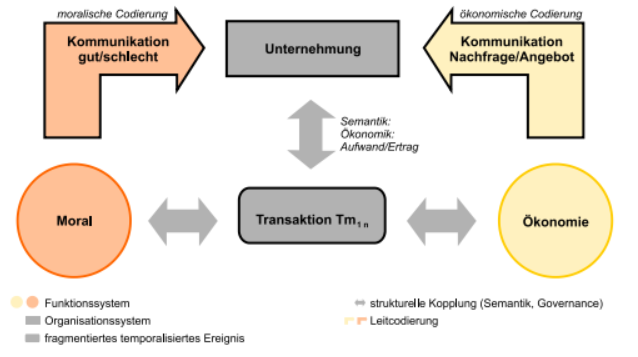
\includegraphics[width=.9\textwidth]{wieland1.png}
\end{center}
Zunächst, so Wieland, hat sich die Gesellschaft aus verschiedenen gleichrangigen und autonomen Funktionensystemen, u.a. der Moral und der Ökonomie, mit ganz spezifischen binären Leitcodes herausgebildet. So kommuniziert das ökonomische Funktionssystem rein ökonomisch mit Angebot und Nachfrage. Dort wo der Preis am niedrigsten ist, wird auch das Produkt gekauft. Anders sieht es bei dem Funktionssystem Moral aus. Dieses codiert die gesellschaftliche Kommunikation, das heißt die Ausgestaltung von Unsicherheiten, in \textit{gut und schlecht} und reduziert Verhalten oder Handlungen auf \textit{zulässig und unzulässig}. Wertschätzung wird bei der Moral durch Zuweisung von \textit{Achtung und Missachtung} begründet. Also wenn der eine Händler Produkte durch Kinderarbeit produzieren lässt und der andere nicht, so ist das Verhalten des einen Händlers moralisch unzulässig und bei dem anderen zulässig. Wenn man jetzt Wielands Ansätzen folgt, so wird ggf. das kostspieligere aber moralisch zulässige Produkt gekauft. Somit hat jede wirtschaftliche Transaktion eine moralische Dimension und wird so durch moralische und ethische Vorstellungen beeinflusst.

\subsection{Wirtschaftliche Transaktionen}
Die moralische Dimension der wirtschaftliche Transaktion ist eine Funktion der individuellen Selbststeuerungsmechanismen der involvierten Personen, der formalen und informalen Institutionen eines gegebenen Umfelds und der Beschaffenheit der Koordinations- und Kooperationsmechanismen einer wirtschaftlichen Organisation.
\[Tm_i=f_{(a\cdot IS_i, b\cdot FI_{ij}, c\cdot IF_{ij}, d\cdot OKK_i)}\]
IS steht für individuelle Selbstbindung oder Selbstgovernance. Selbstbindungsstrategien können auf Prinzipien der Tugend, rationale Vorteilskalküle oder andere Mechanismen zurückgehen.[2] Dieser Punkt ist von Person zu Person unterschiedlich. Zur Verknüpfung mit dem Beispiel der Kinderarbeit, ist es hier Fall, ob und in welcher Weise eine Beitrag zur Abschaffung von Kinderarbeit geleistet werden könnte.\\
FI steht für die formalen Institutionen einer gegeben Gesellschaft. Ein Beispiel wäre hier der Umweltschutz in einer entsprechenden Gesetzgebung anzuführen, die in ihren Bestandteilen zwar spezifisch für die Transaktion sind und für einen bestimmten Ort gilt.
\\
IF steht für die informalen Institutionen einer Gesellschaft, wie religiöse oder moralische Überzeugungen einer gegebenen Kultur. Zum Beispiel ist es allgemein bekannt, dass Korruption und deren moralische Bewertung tief in den kulturellen Grundüberzeugungen verankert ist.\\
Zur guter Letzt steht OKK für die Koordinations- und Kooperationsmechanismen einer bestimmten Organisation, mit denen Transaktionen geführt, gesteuert und kontrolliert werden. Darunter sind Leitlinien und Prozesse zu verstehen, mit denen moralische Anforderungen, wie Verzicht auf Kinderarbeit und Korruption operationalisiert und implementiert werden.\\
Die Koeffizienten a, b, c, d können jeweils den Wert 1, 0 oder – 1 annehmen. Das Vorzeichen informiert darüber, ob und in welcher Weise die oben aufgelisteten Argumente wirksam oder nicht wirksam sind. Der Wert 1 gibt eine positive Wirksamkeit im Hinblick auf die moralische Dimension an. Der Wert -1 gibt genau das Gegenteil an, nämlich eine negative Wirkung auf die moralische Transaktion und der Wert 0 besagt, dass die Wirkung nicht angenommen wird.
\begin{center}
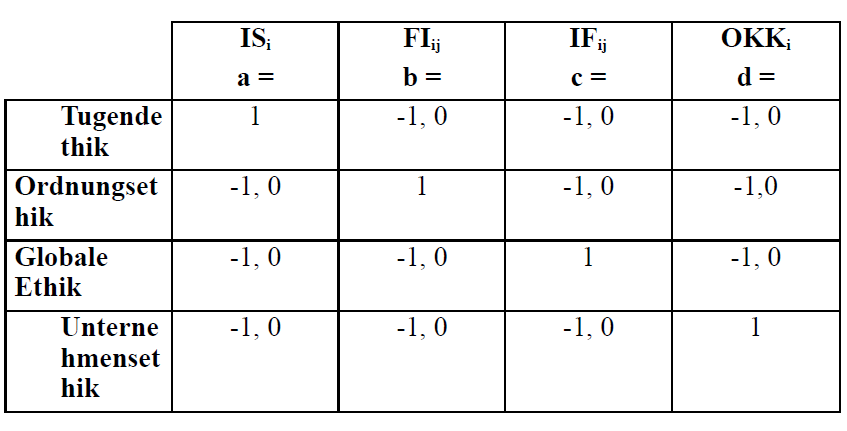
\includegraphics[width=.7\textwidth]{wieland_tabelle.png}
\end{center}


\clearpage
\frontmatter%Stil des Headers/Footers ändern
\renewcommand{\plaintitle}{Literaturverzeichnis}
\pagenumbering{Roman}
\setcounter{page}{3}
\addtocontents{toc}{\vspace{24pt}}
\addcontentsline{toc}{part}{Literaturverzeichnis}%Literatur-Verz. ins Inhaltsverzeichnis
\printMyBibliography


\end{document}